\documentclass[12pt, a4paper, simple]{eskdtext}

\usepackage{hyperref}
\usepackage{env}
\usepackage{_sty/gpi_lst}
\usepackage{_sty/gpi_toc}
\usepackage{_sty/gpi_t}
\usepackage{_sty/gpi_p}
\usepackage{_sty/gpi_u}

% Код
% \ESKDletter{О}{Л}{Р}
% \def \gpiDocTypeNum {81}
% \def \gpiDocVer {00}
% \def \gpiCode {\ESKDtheLetterI\ESKDtheLetterII\ESKDtheLetterIII.\gpiStudentGroupName\gpiStudentGroupNum.\gpiStudentCard-0\gpiDocNum~\gpiDocTypeNum~\gpiDocVer}

\def \gpiDocTopic {Отчёт лабораторной работы №\gpiDocNum}

% Графа 1 (наименование изделия/документа)
% \ESKDcolumnI {\ESKDfontII \gpiTopic \\ \gpiDocTopic}

% Графа 2 (обозначение документа)
% \ESKDsignature {\gpiCode}

% Графа 9 (наименование или различительный индекс предприятия) задает команда
% \ESKDcolumnIX {\gpiDepartment}

% Графа 11 (фамилии лиц, подписывающих документ) задают команды
% \ESKDcolumnXIfI {\gpiStudentSurname}
% \ESKDcolumnXIfII {\gpiTeacherSurname}
% \ESKDcolumnXIfV {\gpiTeacherSurname}

\begin{document}
    \begin{ESKDtitlePage}
    \ESKDstyle{empty}
    \begin{center}
        \gpiMinEdu \\
        \gpiEdu \\
        \gpiKaf \\
    \end{center}

    \vfill

    \begin{center}
        \gpiTopic
    \end{center}

    \vfill

    \begin{center}
        \textbf{\gpiDocTopic} \\
        ПО ДИСЦИПЛИНЕ \gpiDiscipline \\
    \end{center}

    \vfill

    \begin{flushright}
        \begin{minipage}[t]{7cm}
            Выполнил:\\
            \PageTitleStudentInfo
            \PageTitleDateField
            \hspace{0pt}

            Проверил:\\
            \PageTitleTeacherInfo
            \PageTitleDateField
        \end{minipage}
    \end{flushright}

    \vfill

    \begin{center}
        \PageTitleCity~\ESKDtheYear
    \end{center}
\end{ESKDtitlePage}

    \ESKDstyle{empty}
    \begin{center}
        \textbf{\gpiDocTopic}
    \end{center}

    % = = = = = = = =
    \paragraph{} \textbf{Тема}: <<\gpiTopicRep>>

    \paragraph{} \textbf{Цель}: Научиться создавать приложения, состоящие из нескольких активностей,
    и диалоговые окна, а также познакомиться с элементами тач-интерфейса.

    \paragraph{} \textbf{Что нужно сделать}:

    Научиться создавать многоэкранные приложения. Наследовать MainActivity не от\\ AppCompatActivity, а от ListActivity.
    Создать массив ссылок (ArrayAdapter). Создать классы для страниц (Canari.java, Curili.java, Maldivi.java, Philippini.java).
    Перечислить все активности в манифесте (AndroidManifest.xml).
    Сделать, чтобы по нажатию на элемент меню (ArrayAdapter) открывался определённый класс (Canari.java, Curili.java, Maldivi.java, Philippini.java).
    Поключить в классы его дизайн (сanari.xml, curili.xml, maldivi.xml, philippini.xml).

    Научиться создавать диалоговые окна и всплывающие подсказки

    Научиться писать приложения со слайдингом

    \paragraph{} \textbf{Разработка дизайна}:

    \begin{figure}[!h]
        \centering
        \begin{minipage}{0.19\textwidth}
            \centering
            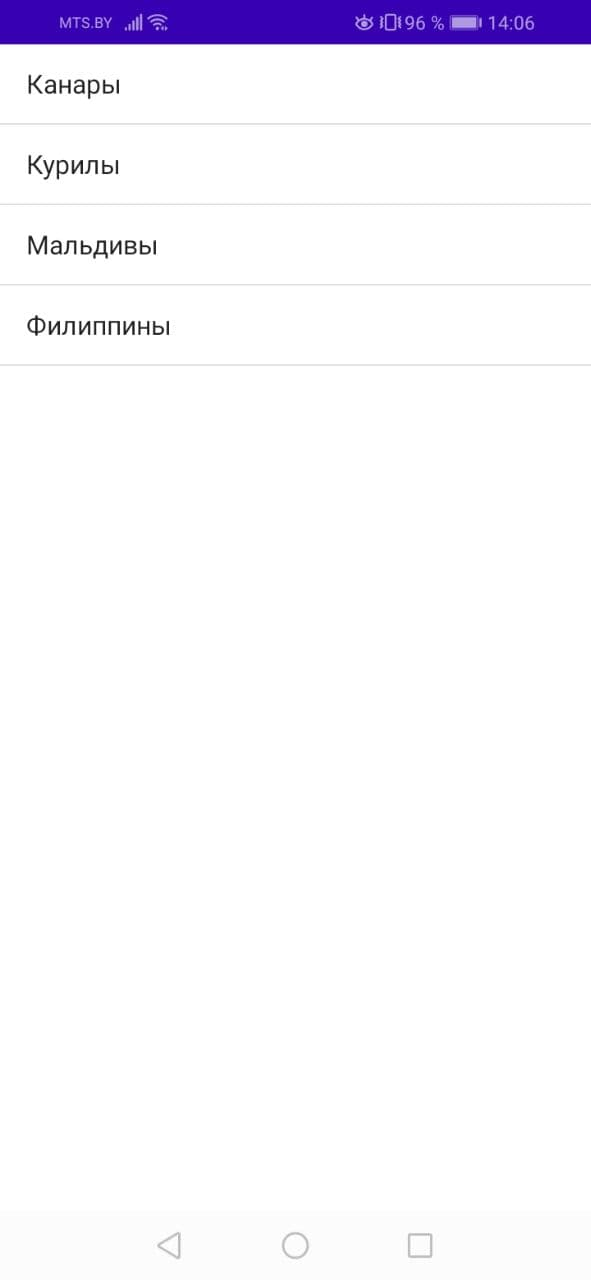
\includegraphics[width=\linewidth]
                {_assets/MultiScreen__MainActivity.jpg}
            \caption{Меню}
            \label{fig:MultiScreen__MainActivity}
        \end{minipage}
        \begin{minipage}{0.19\textwidth}
            \centering
            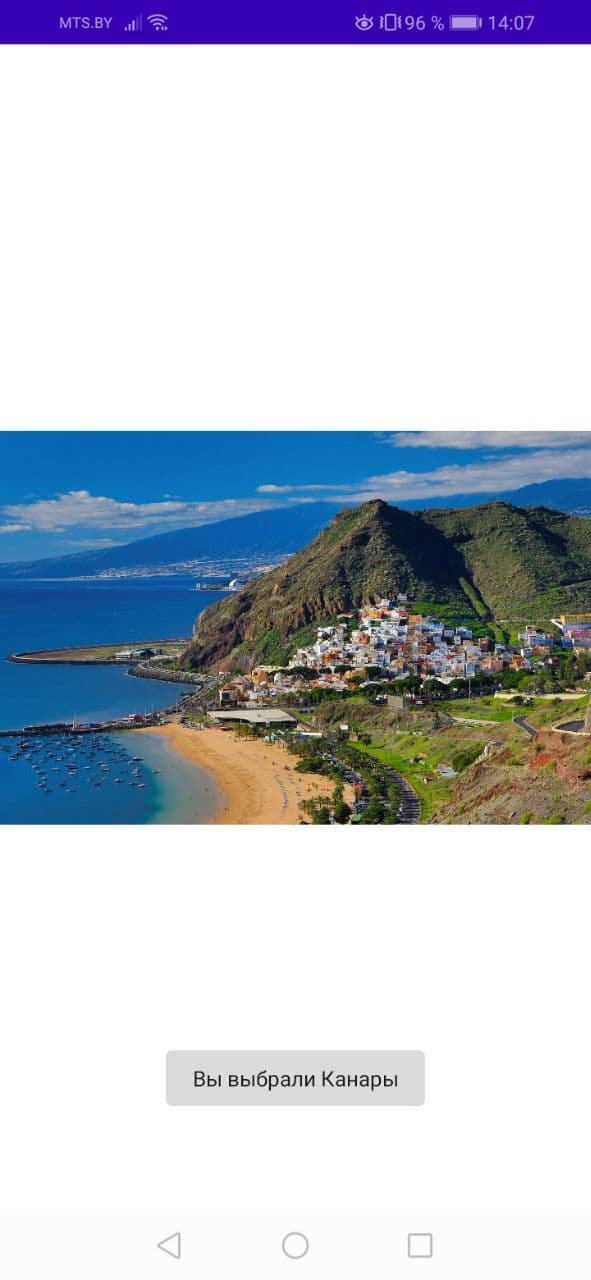
\includegraphics[width=\linewidth]
                {_assets/MultiScreen__Canari.jpg}
            \caption{Канары}
            \label{fig:MultiScreen__Canari}
        \end{minipage}
        \begin{minipage}{0.19\textwidth}
            \centering
            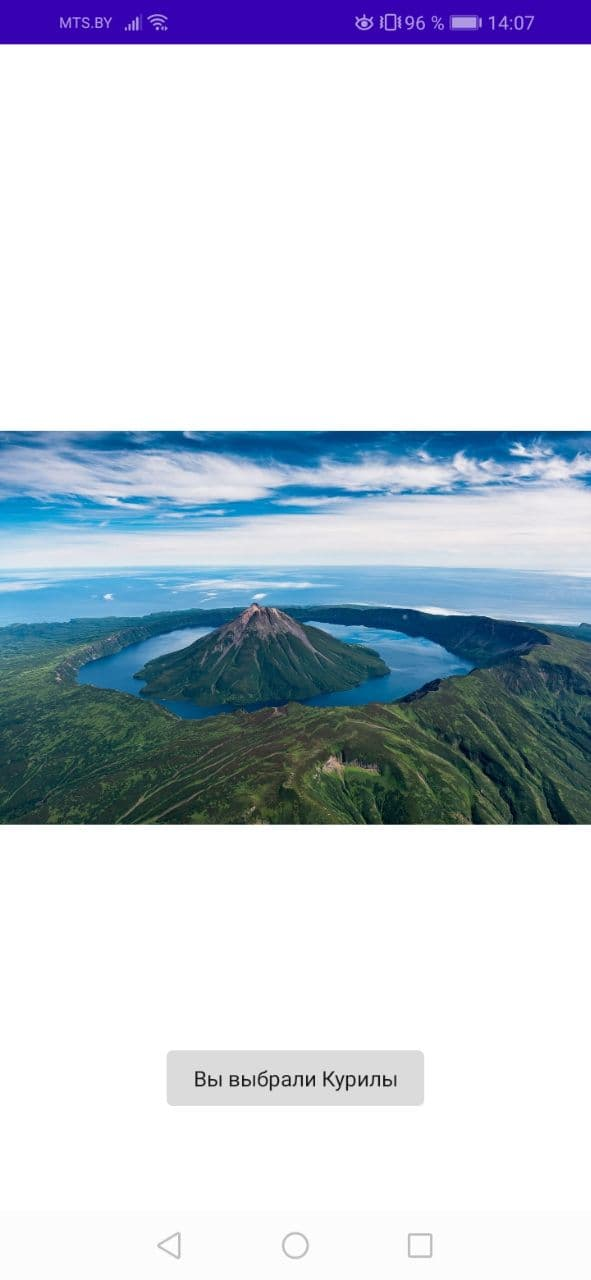
\includegraphics[width=\linewidth]
                {_assets/MultiScreen__Curili.jpg}
            \caption{Курилы}
            \label{fig:MultiScreen__Curili}
        \end{minipage}
        \begin{minipage}{0.19\textwidth}
            \centering
            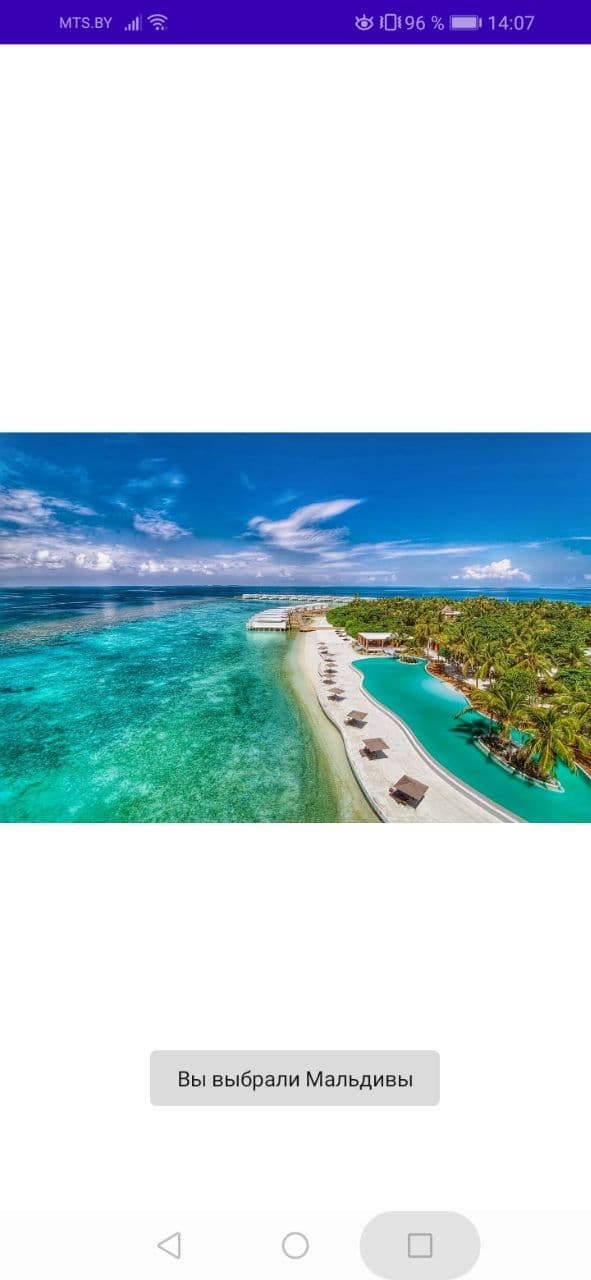
\includegraphics[width=\linewidth]
                {_assets/MultiScreen__Maldivi.jpg}
            \caption{Мальдивы}
            \label{fig:MultiScreen__Maldivi}
        \end{minipage}
        \begin{minipage}{0.19\textwidth}
            \centering
            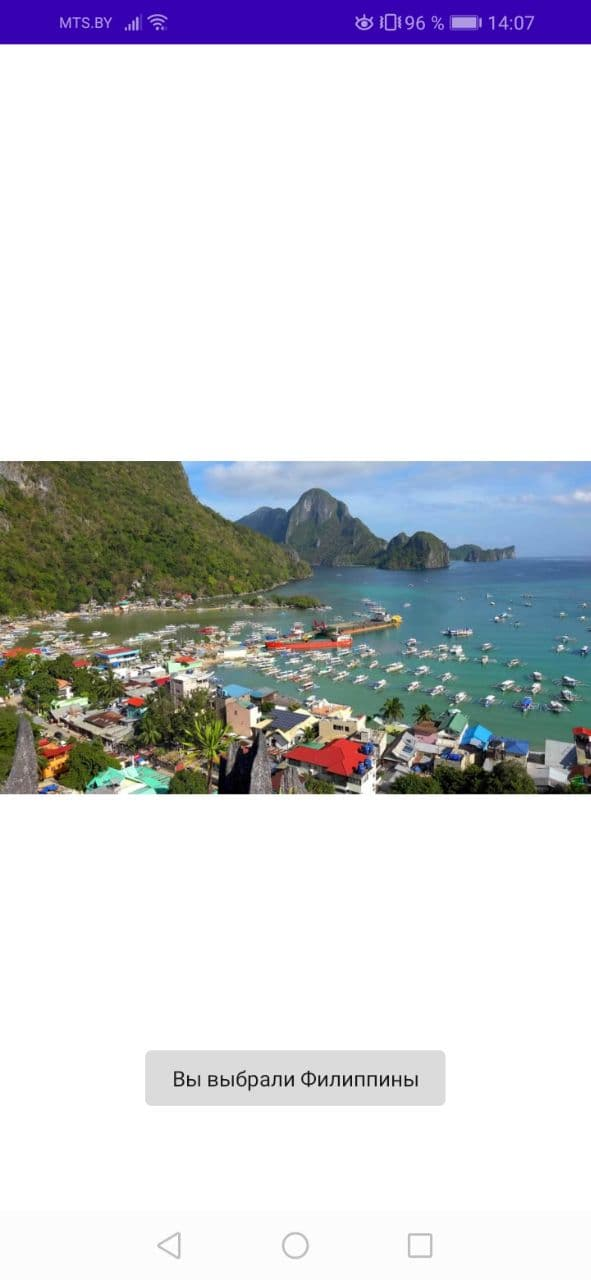
\includegraphics[width=\linewidth]
                {_assets/MultiScreen__Philippini.jpg}
            \caption{Филиппины}
            \label{fig:MultiScreen__Philippini}
        \end{minipage}
    \end{figure}

    \paragraph{} \textbf{Исходный код}: 

    \lstinputlisting[language=java, name=/app/src/main/java/.../MainActivity.java]
        {../gpi_src/gpi_rpodms6_lab6__MultiScreen/app/src/main/java/io/github/Pavel_Innokentevich_Galanin/gpi_rpodms6_lab6__MultiScreen/MainActivity.java}
    
    \lstinputlisting[language=java, name=/app/src/main/java/.../Canari.java]
        {../gpi_src/gpi_rpodms6_lab6__MultiScreen/app/src/main/java/io/github/Pavel_Innokentevich_Galanin/gpi_rpodms6_lab6__MultiScreen/Canari.java}
    \lstinputlisting[language=java, name=/app/src/main/java/.../Curili.java]
        {../gpi_src/gpi_rpodms6_lab6__MultiScreen/app/src/main/java/io/github/Pavel_Innokentevich_Galanin/gpi_rpodms6_lab6__MultiScreen/Curili.java}
    \lstinputlisting[language=java, name=/app/src/main/java/.../Maldivi.java]
        {../gpi_src/gpi_rpodms6_lab6__MultiScreen/app/src/main/java/io/github/Pavel_Innokentevich_Galanin/gpi_rpodms6_lab6__MultiScreen/Maldivi.java}
    \lstinputlisting[language=java, name=/app/src/main/java/.../Philippini.java]
        {../gpi_src/gpi_rpodms6_lab6__MultiScreen/app/src/main/java/io/github/Pavel_Innokentevich_Galanin/gpi_rpodms6_lab6__MultiScreen/Philippini.java}

    \lstinputlisting[language=xml, name=/app/src/main/AndroidManifest.xml]
        {../gpi_src/gpi_rpodms6_lab6__MultiScreen/app/src/main/AndroidManifest.xml}

    \lstinputlisting[language=xml, name=/app/src/main/res/layout/canari.xml]
        {../gpi_src/gpi_rpodms6_lab6__MultiScreen/app/src/main/res/layout/canari.xml}
    \lstinputlisting[language=xml, name=/app/src/main/res/layout/curili.xml]
        {../gpi_src/gpi_rpodms6_lab6__MultiScreen/app/src/main/res/layout/curili.xml}
    \lstinputlisting[language=xml, name=/app/src/main/res/layout/maldivi.xml]
        {../gpi_src/gpi_rpodms6_lab6__MultiScreen/app/src/main/res/layout/maldivi.xml}
    \lstinputlisting[language=xml, name=/app/src/main/res/layout/philippini.xml]
        {../gpi_src/gpi_rpodms6_lab6__MultiScreen/app/src/main/res/layout/philippini.xml}

    \lstinputlisting[language=xml, name=/app/src/main/res/values/strings.xml]
        {../gpi_src/gpi_rpodms6_lab6__MultiScreen/app/src/main/res/values/strings.xml}

    \paragraph{} \textbf{Вывод}:
    
    Наследовали для MainActivity не AppCompatActivity, а ListActivity.
    Создали меню, используяя список ArrayAdapter.
    Создали классы для страниц (Canari.java, Curili.java, Maldivi.java, Philippini.java).
    Перечислили активности в манифесте (AndroidManifest.xml).
    Реализовали меню, которое мо нажатию на элемент открывает определенный класс.
    К каждому классу придумали дизайн (canari.xml, curili.xml, maldivi.xml, philippini.xml).

    % = = = = = = = =
    % \newpage
    % \addcontentsline{toc}{section}{СПИСОК ИСПОЛЬЗОВАННЫХ ИСТОЧНИКОВ}
    % \section*{Список использованных источников}
    \paragraph{} \textbf{Список использованных источников}
    \begin{enumerate}
        \item[1.] Кондратюк, А.П. Разработка приложений для мобильных операционных систем «Android» :
        ЭУМК для студ. второй ступени (магистратуры) специальности 1-31 81 06 <<Веб-программирование и интернет-технологии>>
        физ.-мат. фак. / А.П. Кондратюк ; Брест. гос. ун-т им. А.С. Пушкина, каф. ПМиИ. – Брест :
        электрон. издание БрГУ, 2016. – 469 с.\\
        §21. Лабораторная работа №4, cc. 362-388
        \item[2.] Канары: 2 тыс изображений найдено в Яндекс.Картинках [Электронный ресурс]
        - Режим доступа: \url{https://yandex.by/images/search?text=%D0%9A%D0%B0%D0%BD%D0%B0%D1%80%D1%8B&from=tabbar&pos=9&img_url=https%3A%2F%2Ffunart.pro%2Fuploads%2Fposts%2F2019-11%2F1572810389_kanary-kurort-ispanija-47.jpg&rpt=simage}.
        Дата~доступа:~18.02.2022.
        \item[3.] Курилы: 2 тыс изображений найдено в Яндекс.Картинках [Электронный ресурс]
        - Режим доступа: \url{https://yandex.by/images/search?text=%D0%9A%D1%83%D1%80%D0%B8%D0%BB%D1%8B&from=tabbar&pos=14&img_url=https%3A%2F%2Fscontent-hel2-1.cdninstagram.com%2Fv%2Ft51.2885-15%2Fe35%2F106582006_108071927556132_2724570415950092066_n.jpg%3F_nc_ht%3Dscontent-hel2-1.cdninstagram.com%26_nc_cat%3D100%26_nc_ohc%3DfvuvJPxm7A8AX_rEwEd%26oh%3Dbeaf9d23b67ec9eaab9b4bf2657a2b82%26oe%3D5F71FE88&rpt=simage}.
        Дата~доступа:~18.02.2022.
        \item[4.] Мальдивы: 2 тыс изображений найдено в Яндекс.Картинках [Электронный ресурс]
        - Режим доступа: \url{https://yandex.by/images/search?from=tabbar&text=%D0%9C%D0%B0%D0%BB%D1%8C%D0%B4%D0%B8%D0%B2%D1%8B&pos=6&img_url=https%3A%2F%2Fpbs.twimg.com%2Fmedia%2FC7H04GEXUAEwxep.jpg&rpt=simage}.
        Дата~доступа:~18.02.2022.
        \item[5.] Филиппины: 2 тыс изображений найдено в Яндекс.Картинках [Электронный ресурс]
        - Режим доступа: \url{https://yandex.by/images/search?text=%D0%A4%D0%B8%D0%BB%D0%B8%D0%BF%D0%BF%D0%B8%D0%BD%D1%8B&from=tabbar&p=1&pos=44&rpt=simage&img_url=https%3A%2F%2Fsun9-28.userapi.com%2Fimpg%2FITNNzv7JeYCe2hIvmAkWY3zDYWnl8JQzAKdmmg%2F3mUCeh4opDc.jpg%3Fsize%3D320x240%26quality%3D96%26sign%3D87d3b29a96500ca2a079fff38414dbcf%26type%3Dalbum}.
        Дата~доступа:~18.02.2022.
    \end{enumerate}
    \newpage
\end{document}
